\chapter{Fundamental Ideas}
\section{Introduction}
We assume familiarity with traditional machine learning, basic probability and statistics. We look at why a different perspective
is needed and why deep learning is a suitable alternative.

\section{Traditional Machine Learning}
The older/traditional way of applying machine learning consisted of the following steps:
\begin{enumerate}
    \item \textbf{Feature Extraction:} Features which can be used to discriminate between classes is identified. This step usually requires in-field knowledge about the problem.
    \item \textbf{Model Selection: } A model is selected which trains on the extracted features. Ensable
    methods can be used to boost performance.
    \item \textbf{Cross-validation/Testing: }The model is tested/cross-validated on withheld data to check accuracy and tune hyperparameters.
\end{enumerate}
The drawbacks of this approach are:
\begin{enumerate}
    \item \textbf{Feature Extraction: }This step requires in-field knowledge. It is very difficult to study a
    whole new branch of knowledge for a single problem.
    \item \textbf{Amount of Data: }In the current era, the amount of data sometimes is simply so large
    that it is hard to extract features manually.
    \item \textbf{Unorganized Data: } Feature extraction is hard in unorganized data (such as a text corpus or media inputs like images, audio and videos).
\end{enumerate}
\section{The idea behind a neural network: An intuitive perspective}
The idea is to let the machine learn the important features by itself. For example consider the
problem of recognizing handwritten digits like in figure \ref{hnadwriting}. The machine learns to recognize easy features like say a straight line(highlighted in blue), curved arc(highlighted in red) and
circles(highlighted in green) and how those features combine(Like how two circles form an 8).
\begin{marginfigure}
    \begin{center}
        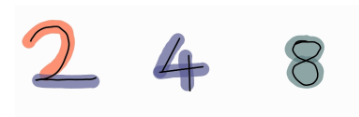
\includegraphics[width=\textwidth]{graphics/handwriting.png}
        \caption{Simple features present in handwritten digits}\label{hnadwriting}
    \end{center}
    \end{marginfigure}
To make an algorithm that can do this we take inspiration from one of the best pattern
learning devices in the world: The human brain$^*$\marginnote{$^*$Taking inspiration from the brain is a repeated theme in deep learning. Those inspirations helped us come up with CNNs and attention mechanisms}. We construct an artificial neuron called a
perceptron. Our idea is each perceptron is responsible for recognizing a single feature: It gives
a high output whenever a feature is present and a low output when it is absent. So if we have
multiple neurons combined, we will be able to recognize complex features that contains many
simpler features that the other neurons have identified.
\section{Ideas behind a neural network: A mathematical perspective}
From a mathematical point of view, there exists a latent space from where the dataset is sampled from. We model the decision boundary in this space using a parametric equation. Then we use already existing data to tune the parameter so that our modelled decision boundary is an estimate of the actual decision boundary.
\section{Comparison between traditional ML and deep learning}
Traditional ML models show better prediction when the amount of features involved is small.
Features can be individually engineered and interpreted. Moreover, such models often provide
more transparency on ow each feature is used and should be preferred when the question of how
the machine a particular conclusion becomes important. Examples include medical domains or
when there is a question of ethics involved.
\begin{marginfigure}
    \begin{center}


        \tikzset{every picture/.style={line width=0.75pt}} %set default line width to 0.75pt        

        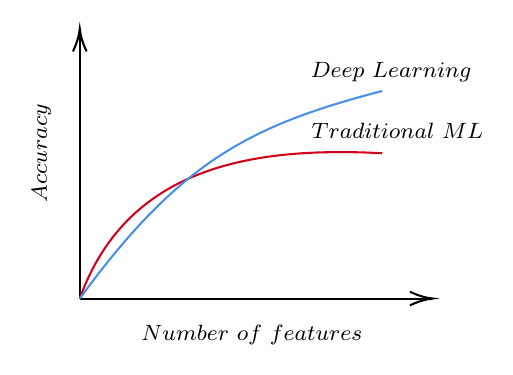
\begin{tikzpicture}[x=0.75pt,y=0.75pt,yscale=-1,xscale=1]
        %uncomment if require: \path (0,300); %set diagram left start at 0, and has height of 300
        
        %Straight Lines [id:da9454167580251368] 
        \draw    (60,180) -- (60,52) ;
        \draw [shift={(60,50)}, rotate = 90] [color={rgb, 255:red, 0; green, 0; blue, 0 }  ][line width=0.75]    (10.93,-3.29) .. controls (6.95,-1.4) and (3.31,-0.3) .. (0,0) .. controls (3.31,0.3) and (6.95,1.4) .. (10.93,3.29)   ;
        %Straight Lines [id:da010275980039295085] 
        \draw    (60,180) -- (228,180) ;
        \draw [shift={(230,180)}, rotate = 180] [color={rgb, 255:red, 0; green, 0; blue, 0 }  ][line width=0.75]    (10.93,-3.29) .. controls (6.95,-1.4) and (3.31,-0.3) .. (0,0) .. controls (3.31,0.3) and (6.95,1.4) .. (10.93,3.29)   ;
        %Curve Lines [id:da007145164916298241] 
        \draw [color={rgb, 255:red, 208; green, 2; blue, 27 }  ,draw opacity=1 ]   (60,180) .. controls (82.5,117.4) and (141.11,106.6) .. (205.71,110) ;
        %Curve Lines [id:da2273240488698708] 
        \draw [color={rgb, 255:red, 74; green, 144; blue, 226 }  ,draw opacity=1 ]   (60,180) .. controls (108.41,113.8) and (142.09,96.6) .. (205.71,80) ;
        
        % Text Node
        \draw (88.2,191.2) node [anchor=north west][inner sep=0.75pt]  [font=\footnotesize]  {$Number\ of\ features$};
        % Text Node
        \draw (169.8,64.8) node [anchor=north west][inner sep=0.75pt]  [font=\footnotesize]  {$Deep\ Learning$};
        % Text Node
        \draw (170.2,94.1) node [anchor=north west][inner sep=0.75pt]  [font=\footnotesize]  {$Traditional\ ML$};
        % Text Node
        \draw (35.4,135) node [anchor=north west][inner sep=0.75pt]  [font=\footnotesize,rotate=-270]  {$Accuracy$};
        
        
        \end{tikzpicture}
        
    \end{center}
\caption{Comparison of accuracy between deep learning and traditional ML methods.}
\end{marginfigure}
Deep learning models are better when data is unstructured or there are a lot of features which
need to be considered. With proper construction and training almost any decision boundaries
can be learned.
\section{The perceptron}
As mentioned before, a perceptron can be thought to be an artificial neuron. We make a simplification and assume that each perceptron is responsible for identifying some pattern $P$. A scheme of what a perceptron looks like is given in \ref{perceptron}
\begin{marginfigure}
    \begin{center}
        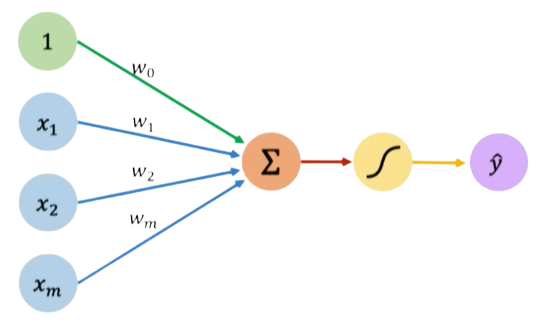
\includegraphics[width=\textwidth]{graphics/nobg perceptron.png}
    \end{center}
    \caption{Schematic diagram of a perceptron,\textit{Src: MIT Introduction to Deep Learning,6.S191,Lec-1}}\label{perceptron}
\end{marginfigure} 
We assume the perceptron returns a high value when it detects $P$. The inputs to a perceptron can be features from known observation or outputs of other neuron. Let the inputs be $x_1,x_2\hdots x_n$. We arrange them neatly in a vector $X=[x_1,x_2,x_3\hdots x_n]$. Each of those $x_i$s can be thought to be the presence and absence of a simpler feature. We take a weighted sum of those inputs to get $s=\sum_{1\leq i\leq n}w_ix_i+w_0$. The intuition is the magnitude of $w_i$ is a measure of the importance of feature $x_i$ and the sign is the direction in which $x_i$ affects the feature which the perceptron is detecting. For example, if the perceptron is detecting if the input is 8 and $x_i$ is the output from another perceptron that detects if a straight line is present then $w_i$ will be negative: there is no straight line in 8. On the other hand,  $x_j$ is the output from another perceptron that detects if a circle is present then $w_i$ will be positive: there are two of them in 8. $w_0$ is just a centering constant. The output of the perceptron will be $y=\sigma(s)$, where $\sigma$ is known as the activation function. 

\section{Chaining Neurons: A simple neural network}
\begin{figure}
    \begin{center}
        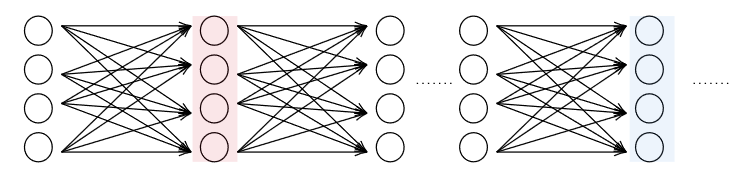
\includegraphics[width=\textwidth]{graphics/nn}
    \end{center}
    \caption{A simple neural network}\label{nn}
\end{figure}
\noindent A very simple neural network is show in \ref{nn}. Each circle represents the output of a perceptron while the arrow pointing to it are the inputs. Each row of neuron is(for example, the blue or the red
box) called a layer and the layers between the input and output layer are called hidden layers.
The layers on the left(For example, the red layer) learns the simpler features while the layers on the
right(For example, the blue layer) learns more complex features, which is composed of multiple
simpler features.
\section{Non-linearity of the activation function}
Ideally, we want our activation function to be non-linear. A simple calculation shows if the activation function for all perceptrons are 
linear then even if you use multiple layers the output will be a linear combination of the input.
Therefore, we use non-linear activation functions to capture non-linear dependencies between the
input features/ simpler patterns. From a more mathematical perspective, we wish to transform the latent space in a way so that the decision boundaries are linear. This is a common idea when we deal with the question of on
which "side" of a hypersurface does a point lie in. For example, if our latent surface is $\mathbb R^2$ and
the decision boundary is given by some nicely parameterized curve $\gamma$ (Some examples of a
nice $\gamma$ are $x^2 + y^2 - r^2 = 0,mx + c - y = 0, p(x) - y = 0$ where p is polynomial) then the two
sides of gamma are given by $\gamma^{-1}(-\infty, 0)$ and $\gamma^{-1}(0, \infty)$. An example showcasing this is given
in \ref{non-linearity}
\begin{figure}
    \begin{center}
        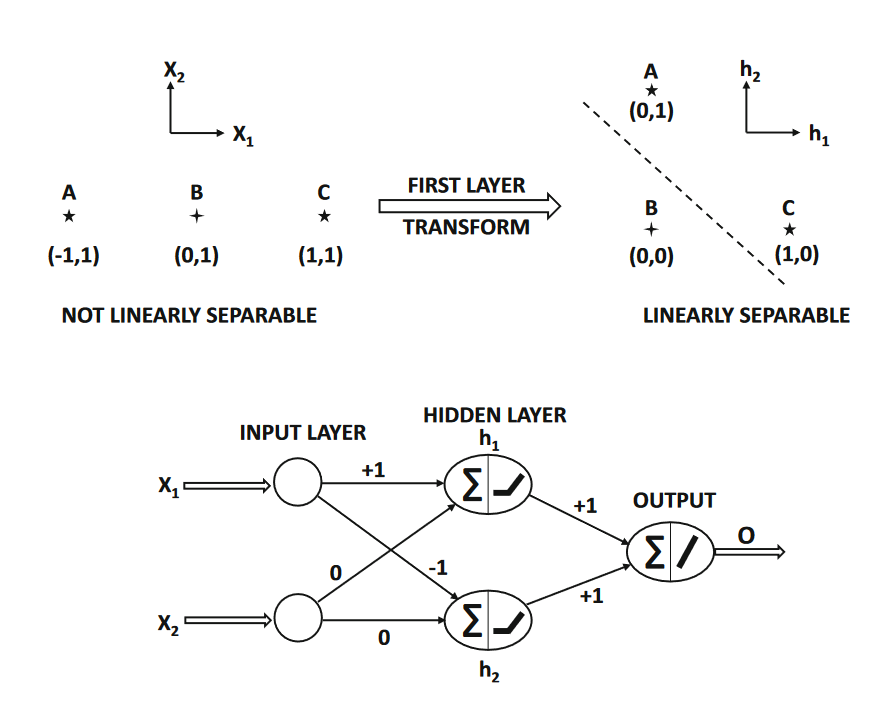
\includegraphics[width=\textwidth]{graphics/non-linearity.png}
    \end{center}
    \caption{A representation of how a non-linear activation function transforms the latent space to give linear boundaries\citep{aggarwal2018neural}}\label{non-linearity}
\end{figure}
\section{Inputs and outputs to a neural network}
\subsection{Classification problem with tabular dataset}
Suppose you have an observation where given features $X=[x_1,x_2\hdots]$ you need to predict the label $Y$. First we replace all categorical $x_i$ and $Y$ with their one hot representation$^{*}$\marginnote{$^{*}$Given categories $c_1,c_2,c_3\hdots c_m$, if $x_i$ belongs to category $c_k$ then in a one hot representation, we represent $x_i$ by $e_k$ where $e_k$ is the $k^{th}$ vector in the standard basis}. If $X$ can take  one $l$ labels (number of possible choices of $Y$), then the second to last layer and the last layer both  have $l$ nodes. If the output from the second to last layer is $y$, at the last layer we take a softmax defined by:
$$\hat Y_i=\frac{\exp(y_i)}{\sum_{1\leq i\leq l}\exp(y_i)}$$
The softmax function maps $\mathbb R^n\to [0,1]^n$ and the interpretation is $\hat Y_i=P(X$ has the label $i)$[Note, by definition $\hat Y_i\in[0,1]$ and  $\sum \hat Y_i=1$]. Softmax is quite expensive to compute. Depending on the problem, we might replace it with other scoring system where a higher $\hat Y_i$ in the output layer means a higher probability that $X$ is in class $i$.

\subsection{Problems where the input is unstructured data}
If the data is unstructured, we use embedding mechanisms to represent them as points in some $\mathbb R^n$ in such a way that similar entries are closer together. Then we proceed as usual. 
\subsection{Regression tasks}
In regression problems, the output $\hat Y$ is simply an estimate of $Y$.


